\chapter{CAWI Mark-up Language}\label{ch:cawiLanguage}	
			This Chapter presents \gls{cawiml} as an alternative authoring language to specify questionnaires only using standard \gls{xml} schema languages. Particularly, it uses a state-transition paradigm for question's sequence and is intended to facilitate the questionnaire routing logic more adequately than the popular hierarchical model. \gls{rpn}, is the expression formalism utilised for describing routing and personalisation constructs indistinctly.

	The rest of this Chapter is structured as follows: Section \ref{sec:cawiLanguage:stateTransition} introduces the state-transition routing structure. Section \ref{sec:cawiLanguage:rpn} explains the postfix notation mode as the formalism for questionnaire expressions, followed by Section \ref{sec:cawiLanguage:xmlLanguage} that explains our \gls{xml} authoring solution. Finally, \gls{xml} details for content, routing and personalisation constructs expressed in \gls{cawiml} are presented in Section \ref{sec:cawiLanguage:cawiml}.
	\section{The State-Transition Modelling Solution}\label{sec:cawiLanguage:stateTransition}
			The state-transition modelling approach is our proposal to better address the routing requirements involving design-code equivalence and adaptability criteria (see Section \ref{sec:literature:flowParadigm}). This model, widely used for the specification of reactive systems \cite{tech:androutsopoulos08}, is inspired by the \gls{efsm} \cite{book:alagar11}.

	An example of the state-transition model, represented in Figure \ref{fig:design:stateTransition}, describes the questionnaire presented in Figure \ref{fig:background:survey}. It contains various types of states, represented by ellipses, that are linked through transitions to form state models (e.g. the Outer and Inner rectangles). 

	Each state model contains variables that reference questions defined in a section (e.g. INF1, Q1, Q2, Q3, Q4, Q5, INF2 and END for the Outer section or Q6a for the Inner). The scope of these is local to a state model and therefore their references do not exist outside. In order to reference variables through any state model, this paradigm defines global place holders, known as fields, that permit sharing data across different parts of a questionnaire (e.g. HAD\_CAR describing an integer number of cars that the respondent had).

	The states are addressed to perform single operations and these may be categorised as follows:

	\begin{itemize}
		\item \emph{Simple} states are used to present the questions to the respondent and to store responses in variables (e.g. every state prefixed with 's').
		\item \emph{Composite} states refer to a defined state model (e.g. c0 and c1 for Outer and Inner state models respectively) and are useful for reducing coupling among questions in a survey.
		\item Pseudo states are normally used to take routing path decisions through the evaluation of boolean expressions. Specifically, there are \emph{if} and \emph{for} states to decide the conditions under which questions are asked and \emph{check} states to validate inconsistent responses. Additionally, the \emph{computation} state unlike its counterparts is utilised to update place holder variables through \emph{arithmetic} expressions.
	\end{itemize}

	The transitions connect a state source with a state target to create a questionnaire's flow (e.g. arrows connect ellipses). If a transition does not define a boolean expression, it is assumed true whenever the state source of the transition is reached. In contrast, if a boolean expression is defined, this means that the expression has to be evaluated in order to determine its truth (e.g. Q1 '01' IS\_SEL Q1 '02' IS\_SEL OR Q1 '03' IS\_SEL OR). Here we propose the use of postfix notation mode as the expression formalism for all the expressions used in the design of a questionnaire.

	The state models have an initial state that determines what state is executed first (e.g. s0 and s8 for Outer and Inner respectively) as well as one or more ending states (e.g. 'sink0', 'sink1' or 'sink2'). Similarly, the state-transition model requires a state model that marks the beginning, i.e. an entry point for the model to capture a questionnaire's flow (e.g. 'c0' and 'sink0' states).

	%Our model reacts to a two types of events: \emph{external}, which occurs whenever a respondent requests moving forward or backward through a questionnaire; and \emph{internal} that is triggered every time a variable is updated. This updating forces an automatic re-evaluation of every expression that contains a reference to that variable. This is possible as X adopts the Observer pattern design implementation. %(see Appendix \ref{sec:design:observerPattern}).

	Accordingly, we formalise the state-transition model that is applied to questionnaire routing as follows:

	\begin{equation}\label{design:eqn:stateTransition}
		M = \langle Q,V,T,I,E \rangle
	\end{equation}
	where,
	\begin{enumerate}
		\item $Q(\neq \emptyset)$ is a finite set of states.
		\item $V$ is the set of state variables. Every variable $x \in V$ may be accessed at every state $q \in Q$.
		\item $T$ is a finite set of transitions. A transition $t \in T$ is represented as $q \xrightarrow{[c]} 
		q'$, where $\{q,q'\} \in Q$ and c is a boolean expression involving variables of $V$ defined in pre-state \emph{q}. The absence of $c$ is interpreted to true.
		\item $I\subset Q$ is the set of initial states. Every composite state has an initial state and consequently there is a set of initial states if the model contains composite states.
		\item $E\subset Q$ is the set of end states. These states may be \emph{sink} addressed to finish a state model or \emph{terminate} to interrupt and finish the execution of a state-transition model.
	\end{enumerate}

	\begin{figure}[H]
	\centering
	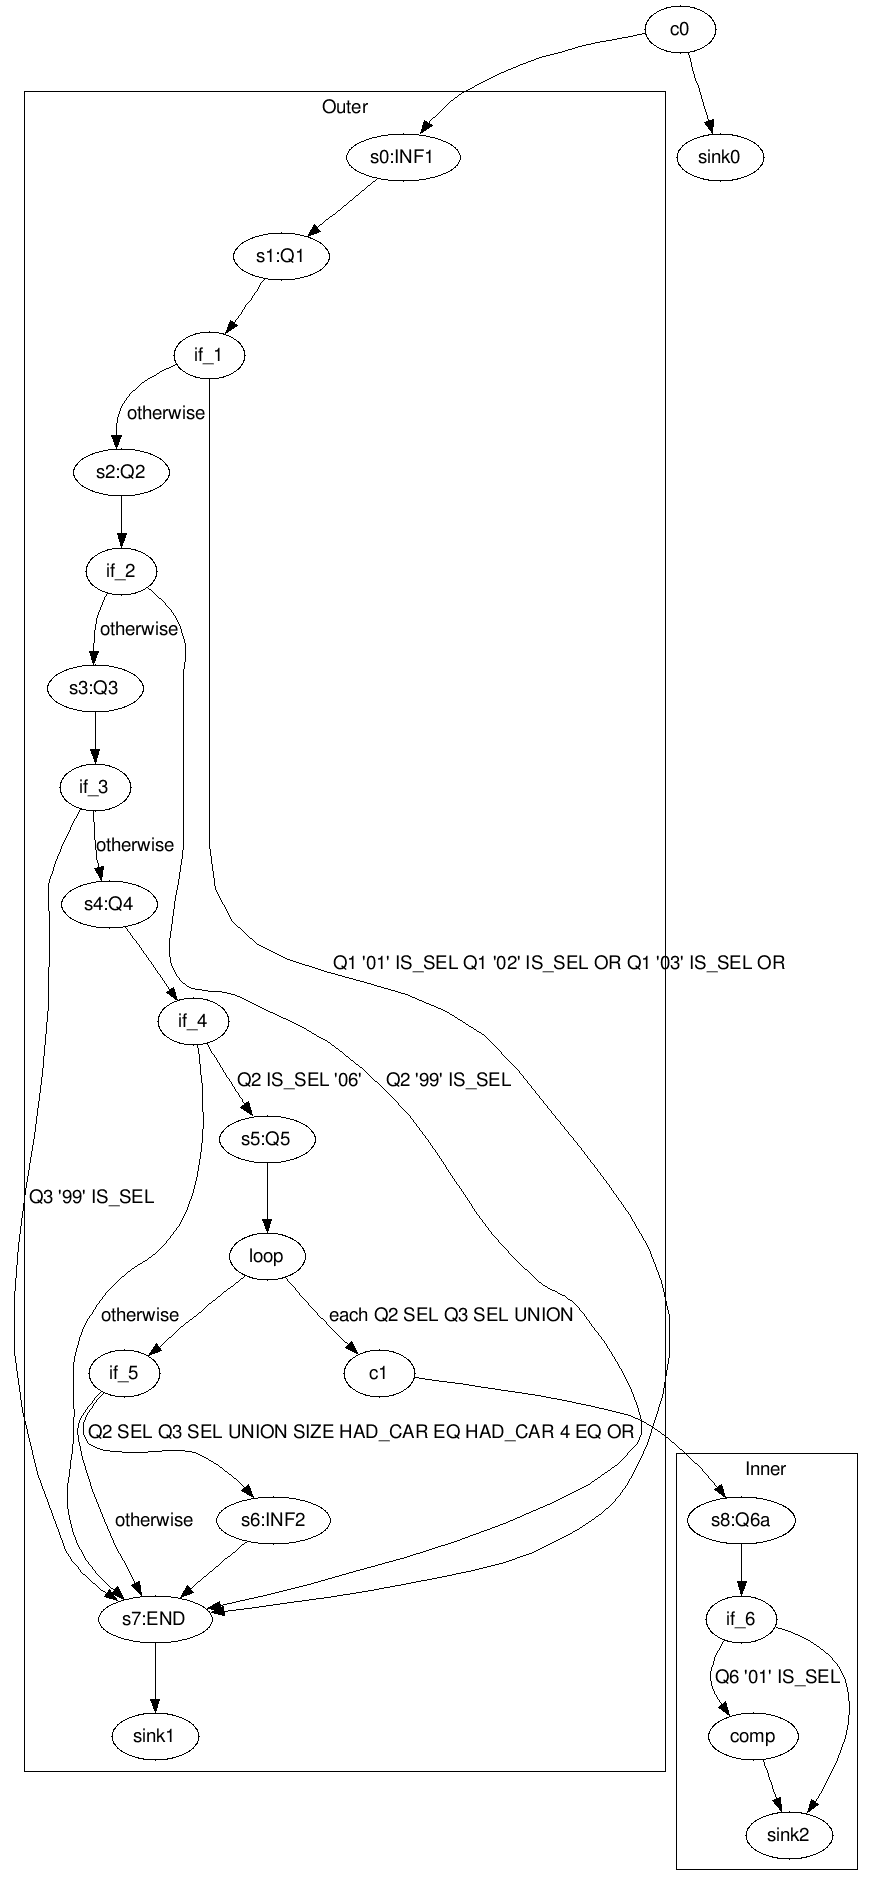
\includegraphics[max size={\textwidth}{\textheight}]{design/img/stateTransition.png}
	\caption{State-Transition for the paper questionnaire in Figure \ref{fig:background:survey}}
	\label{fig:design:stateTransition}
	\end{figure}

	%Our proposal for modelling questionnaire's routing does not explicitly defines skip constructs but it does not mean that the task of negating expressions has to be performed since this model does not rely on sequence lines which allows moving from one state to another by using transitions. Also as there is no possibility to define parent-child hierarchies among states, this potentially reduces the coupling of the routing constructs.

	





	\section{The RPN Notation}\label{sec:cawiLanguage:rpn}
		    The postfix notation, also known as \gls{rpn}, is the notation formalism that we have adopted to define the logical and arithmetical expressions applicable not only for routing constructs such as filters, loops, checks and computations but also for describing text-fill and carry-forward personalisation constructs. Its simplicity to evaluate any kind of expression, the non-ambiguity for operators precedence and its efficiency in terms of number of operations to perform, make this formalism significantly better than infix or prefix modes (see Section \ref{sec:literature:expressionNotation}). The \gls{rpn} formalism has two types of operations: \emph{unary}, that expect one and only one operand; and \emph{binary} which require two operands. By combining these two categories, it is possible to express from simple to complex questionnaire logic constructs.

    Table \ref{tab:design:rpnunary} lists the set of unary operators that \gls{cawiml} provides to express typical questionnaire constructs. The last four operators (e.g. \emph{SEL}, \emph{UNSEL}, \emph{ALL} and \emph{VALUEOF}) are particularly useful for operations carried out through piping constructs. For instance, Figure \ref{fig:background:survey} specifies a carry-forward piping to populate the unselected answers for Q2 as part of responses for Q3 (e.g. Q2 UNSEL). Similarly, the example questionnaire describes a text-fill construct for the Q6a text. This piping feature, which may be formally expressed as ITERATOR VALUEOF, describes the current loop iterator value since Q6a may be executed multiple times during the process of conducting an interview.

    \begin{table}
    \begin{center}
    \begin{tabular}{|c|c|c|}
    \hline 
    \textbf{Name} & \textbf{Operand 1} & \textbf{Result}\tabularnewline
    \hline 
    \hline 
    \textbf{POS} & Integer/Decimal & Integer/Decimal\tabularnewline
    \hline 
    \textbf{NEG} & Integer/Decimal & Integer/Decimal\tabularnewline
    \hline 
    \textbf{INC} & Integer & Integer\tabularnewline
    \hline 
    \textbf{DEC} & Integer & Integer\tabularnewline
    \hline 
    \textbf{NOT} & Boolean & Boolean\tabularnewline
    \hline 
    \textbf{EMPTY} & String/List & Boolean\tabularnewline
    \hline 
    \textbf{SIZE} & String/List & Integer\tabularnewline
    \hline 
    \textbf{SEL} & List & List\tabularnewline
    \hline 
    \textbf{UNSEL} & List & List\tabularnewline
    \hline 
    \textbf{ALL} & List & List\tabularnewline
    \hline 
    \multirow{4}{*}{\textbf{VALUEOF}} & String & \multirow{4}{*}{String}\tabularnewline
    \cline{2-2} 
     & Integer & \tabularnewline
    \cline{2-2} 
     & Decimal & \tabularnewline
    \cline{2-2} 
     & List & \tabularnewline
    \hline 
    \end{tabular}
    \caption{Unary Operators of CAWIML}
    \label{tab:design:rpnunary}
    \end{center}
    \end{table}

    The set of binary operator constructs are listed in Table \ref{tab:design:rpnbinary} and differentiates the operations into four subtypes:
    \begin{itemize}
        \item \emph{equality and relational}, used for conditional statements such as filter, loop or check;
        \item \emph{conditional}, utilised to join two boolean expressions;
        \item \emph{arithmetical}, for operations such as addition, subtraction, multiplication or division; and
        \item \emph{list} to perform operations like UNION or INTERSECTION of sets.
    \end{itemize}

    The commonly used binary operator \emph{IS\_SEL}, checks whether or not a response from a single, multiple or grid question has been chosen. Operators such as UNION or INTERSECTION are crucial to express personalisation features such as complex carry-forward constructs as these permit the join of selected, unselected or all responses from different question types (like single or multiple).

    \begin{sidewaystable}
    \begin{center}
    \begin{tabular}{|c|c|c|c|c|}
    \hline 
    \textcolor{blue}{Type} & \textcolor{blue}{Name} & \textcolor{blue}{Operand 1} & \textcolor{blue}{Operand 2} & \textcolor{blue}{Result}\tabularnewline
    \hline 
    \hline 
    \multirow{7}{*}{\textcolor{blue}{Equality and Relational}} & \multirow{2}{*}{\textbf{EQ}} & String & String & Boolean\tabularnewline
    \cline{3-5} 
     &  & Integer/Decimal & Integer/Decimal & Boolean\tabularnewline
    \cline{2-5} 
     & \multirow{2}{*}{\textbf{NE}} & String & String & Boolean\tabularnewline
    \cline{3-5} 
     &  & Integer/Decimal & Integer/Decimal & Boolean\tabularnewline
    \cline{2-5} 
     & \textbf{LT} & Integer/Decimal & Integer/Decimal & Boolean\tabularnewline
    \cline{2-5} 
     & \textbf{LE} & Integer/Decimal & Integer/Decimal & Boolean\tabularnewline
    \cline{2-5} 
     & \textbf{GT} & Integer/Decimal & Integer/Decimal & Boolean\tabularnewline
    \hline 
    \multirow{2}{*}{\textcolor{blue}{Conditional}} & \textbf{OR} & Boolean & Boolean & Boolean\tabularnewline
    \cline{2-5} 
     & \textbf{AND} & Boolean & Boolean & Boolean\tabularnewline
    \hline 
    \multirow{5}{*}{\textcolor{blue}{Arithmetical}} & \textbf{ADD} & Integer/Decimal & Integer/Decimal & Integer/Decimal\tabularnewline
    \cline{2-5} 
     & \textbf{SUB} & Integer/Decimal & Integer/Decimal & Integer/Decimal\tabularnewline
    \cline{2-5} 
     & \textbf{MUL} & Integer/Decimal & Integer/Decimal & Integer/Decimal\tabularnewline
    \cline{2-5} 
     & \textbf{DIV} & Integer/Decimal & Integer/Decimal & Integer/Decimal\tabularnewline
    \cline{2-5} 
     & \textbf{MOD} & Integer & Integer & Integer\tabularnewline
    \hline 
    \multirow{3}{*}{\textcolor{blue}{List}} & \textbf{IS\_SEL} & List & String & Boolean\tabularnewline
    \cline{2-5} 
     & \textbf{UNION} & List & List & List\tabularnewline
    \cline{2-5} 
     & \textbf{INTERSECTION} & List & List & List\tabularnewline
    \hline 
    \end{tabular}
    \caption{Binary Operators of CAWIML}
    \label{tab:design:rpnbinary}
    \end{center}
    \end{sidewaystable}
   

	\section{The XML Language Solution}\label{sec:cawiLanguage:xmlLanguage}
			The limitations for all grammar-based \gls{xml} language solutions reviewed (see Section \ref{sec:literature:schemaLanguages}) require the use of programming languages to validate semantics for questionnaire specifications. These restrictions have led us to design and implement a new authoring language that is non-proprietary, platform independent and use standard formalisms to define structure, data-types, integrity constraints and business rules. This language, uses the state-transition model for routing logic (see Section \ref{sec:cawiLanguage:stateTransition}) together with \gls{rpn} notation to define expressions either for routing or personalisation constructs (see Section \ref{sec:cawiLanguage:rpn}).  

	\gls{cawiml} uses \gls{xsd} to define structure and data types together with \gls{sch} to express integrity constraints and business rules. We have chosen \gls{xsd} due to its well-defined patterns to express vocabulary and structures, its rich set of data-types, its use of \gls{xml} to define constraints and because it is the recommendation schema formalism proposed by \gls{w3c} (see Section \ref{sec:background:xsd}). \gls{sch} adheres to standard \gls{iso}/\gls{iec} 19757 and is also the only rule-based schema language known to address the semantics limitations that grammar-based languages have through XPath query language (see Section \ref{sec:background:sch}). Therefore, to ensure the correctness of \gls{xml} questionnaire instances, we employ a two step process to integrate four different levels of validation. Figure \ref{fig:design:xmlValidation} describes how this process is carried out.

	\begin{figure}[h]
	\centering
	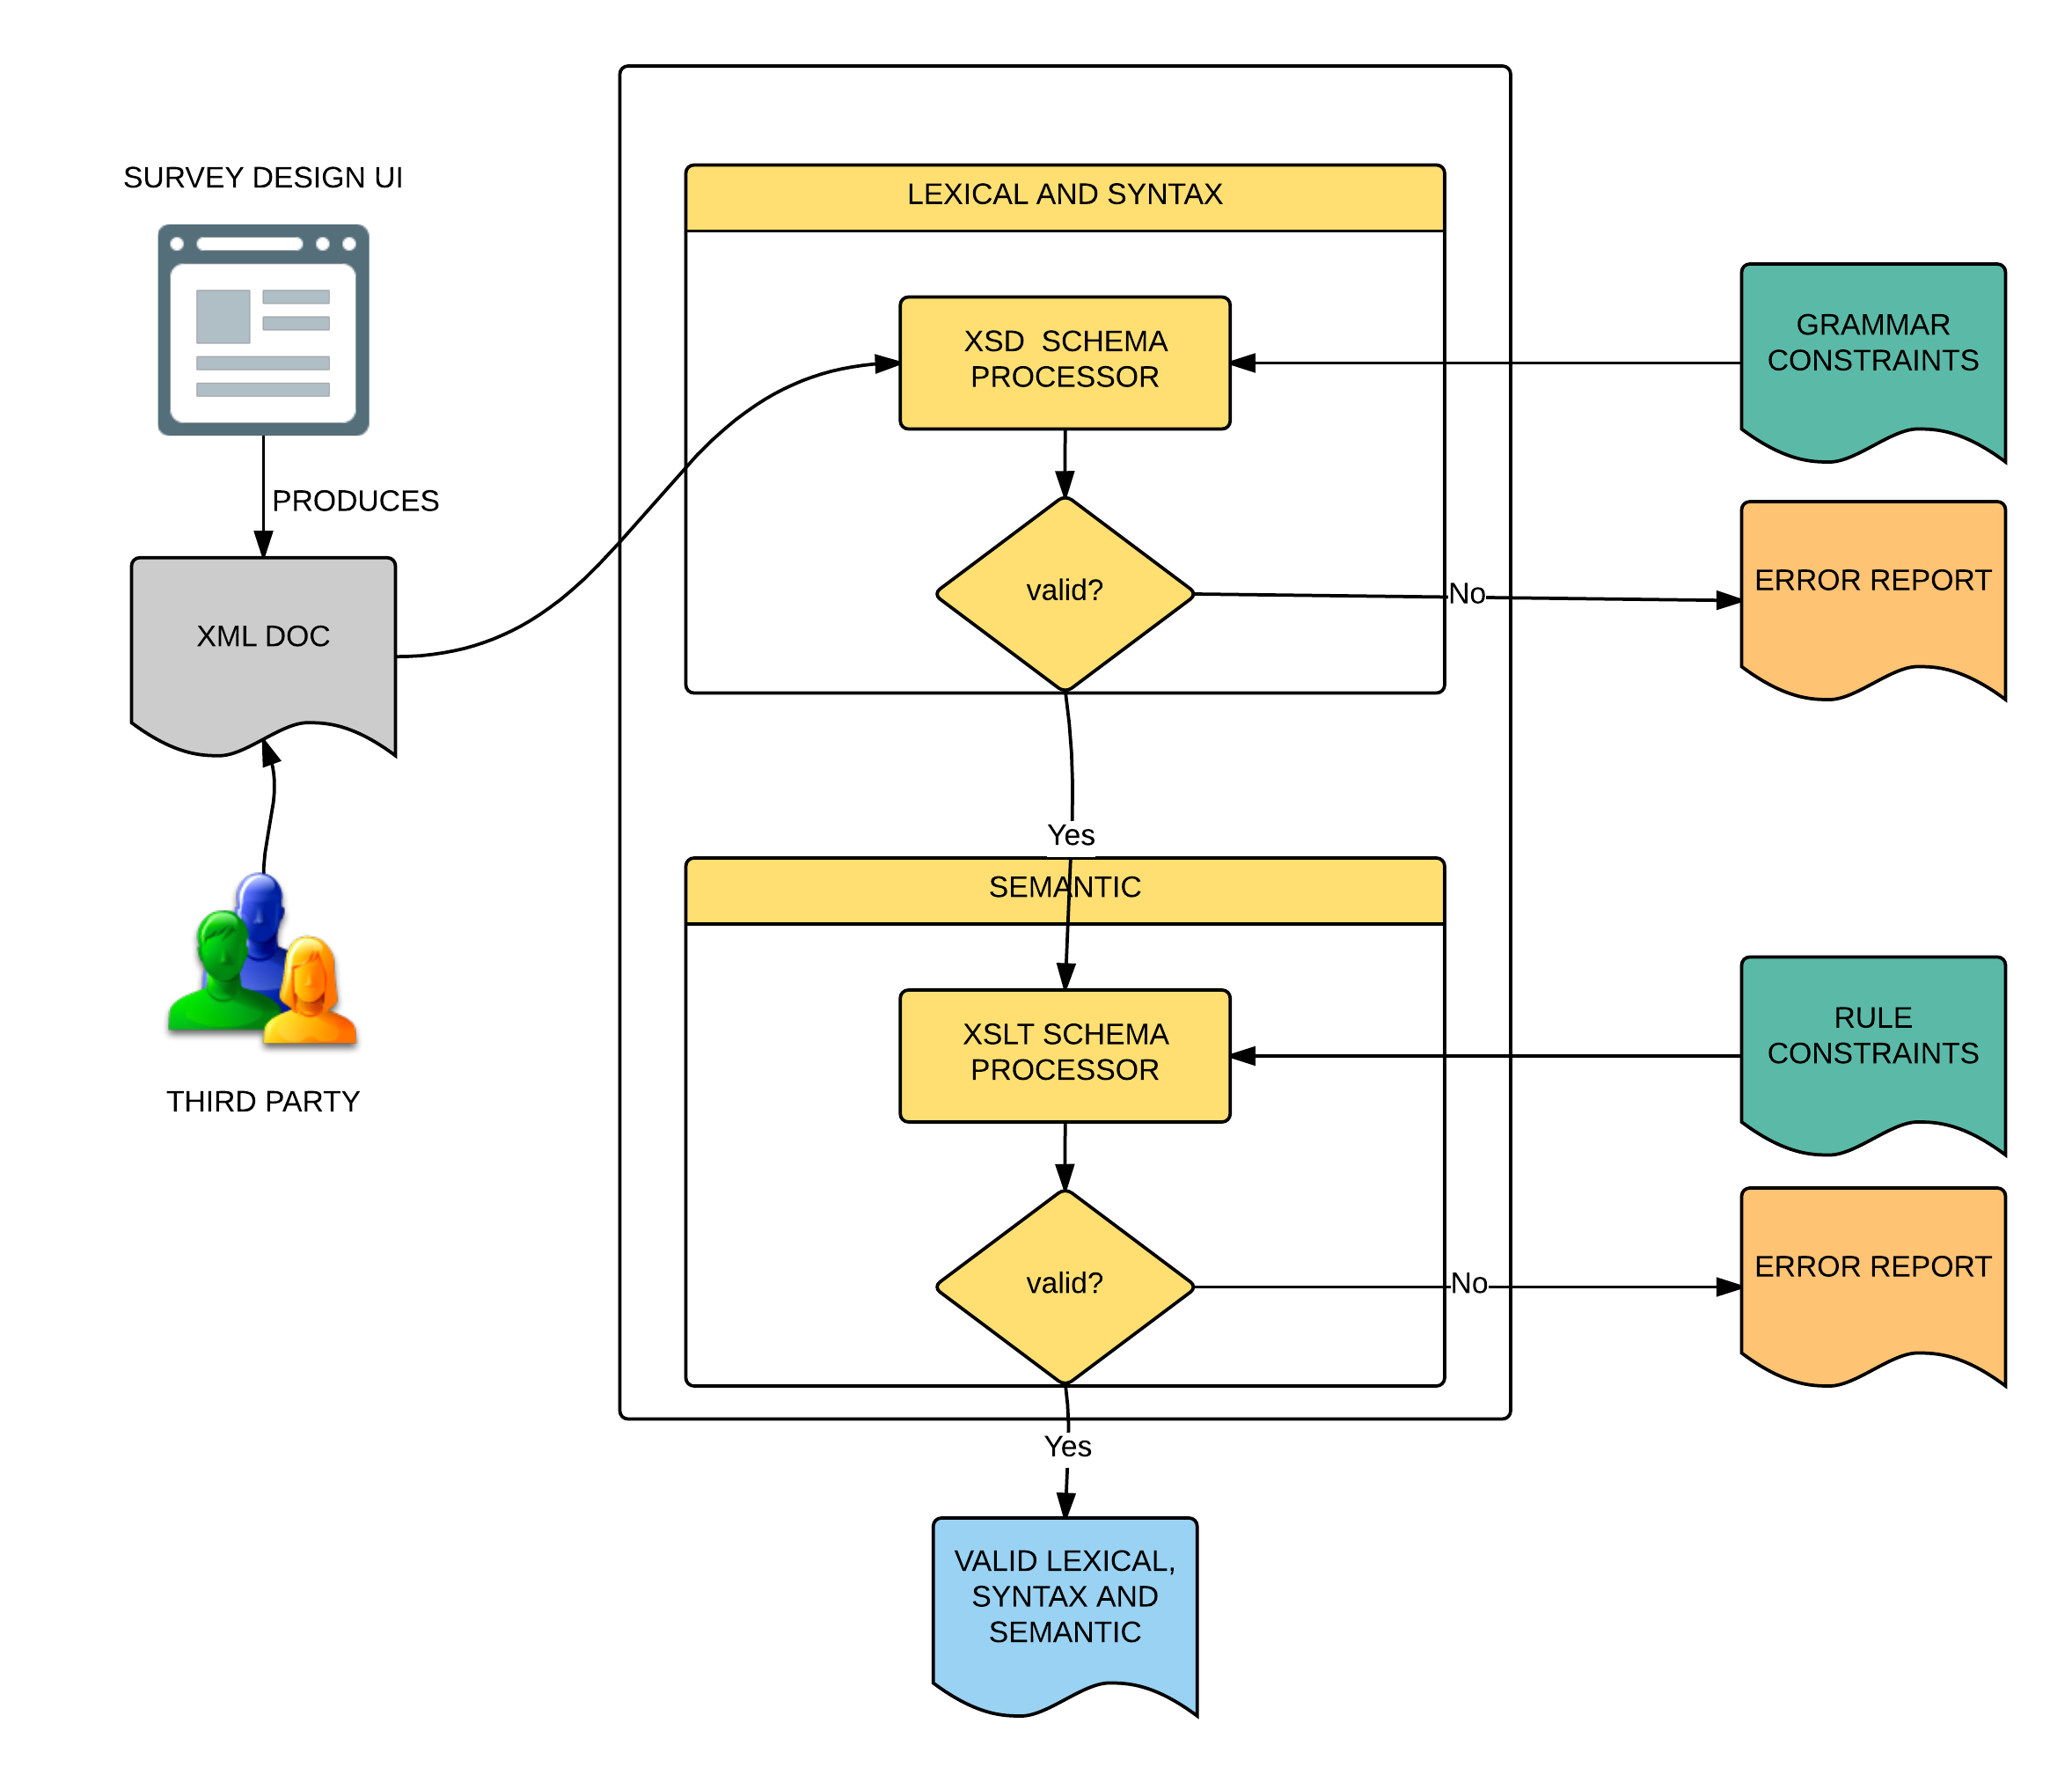
\includegraphics[max size={\textwidth}{\textheight}]{design/img/xmlValidation.png}
	\caption{Validation process of CAWIML}
	\label{fig:design:xmlValidation}
	\end{figure}

	An \gls{xml} document, that is presented either from our interface for designing questionnaires or from any third party, is passed to the validation component. In the first instance, the \gls{xml} schema processor takes our grammar constraints and an \gls{xml} document to verify whether the vocabulary, structures and data-types are valid. Two types of errors can arise from this operation, \emph{non-recoverable} errors that halt the process, i.e. the document is not well-formed (see Section \ref{sec:background:xml}) or \emph{recoverable} which are queued without interrupting the \gls{xml} processing.

	In the second instance, an \gls{xslt} processor takes our \gls{sch} rules, previously converted to the valid format accepted from this processor (see Section \ref{sec:background:sch}), and the \gls{xml} document to determine whether or not the relationships and domain specific rules are correct. The absence of any error at this stage confirms that the \gls{xml} document is valid according to our structure, data-types, integrity constraints and business rules and it is consequently ready to be parsed in our \gls{cawi} system for conducting the on-line survey.

	%We have found during the implementation that the reporting of errors is significantly less predictable for the the grammar-rules since \gls{xsd} schema only produces messages suited for debugging purposes \cite{masterthesis:madsen09}, being difficult to understand for people without any knowledge on schema languages. In contrast, \gls{sch} schema has permitted us to define customised messages that are more user-friendly and better suited for production environments.

	




	\section{CAWIML Language Details}\label{sec:cawiLanguage:cawiml}
			\gls{cawiml} addresses the content, routing and personalisation constructs of surveys by structuring \gls{xml} documents into 5 categories:

	\begin{enumerate}
		\item \emph{Survey} element defines global information relative to a questionnaire and contains information such as name, description and date.
		\item \emph{Content} specifies questions grouped through sections. It provides support for the common question types such as intro, single, multiple, open and grid questions.
		\item \emph{Field} element defines place holders variables needed to share information across different questionnaire sections. String, integer, decimal and list are the types supported currently.
		\item \emph{Routing} captures questionnaire's flow using the state-transition structure proposed in Section \ref{sec:cawiLanguage:stateTransition}.
		\item \emph{Personalisation} defines constructs to adapt questionnaires for an interviewee through features such as text-fill, carry-forward, randomising and rotating.
	\end{enumerate}

	Listings \ref{code:impl:globalStructure} represents the necessary elements to create a specification in \gls{cawiml}. The following sections, showcase the content, routing and personalisation categories.

	\lstinputlisting[caption={CAWIML global structure},label={code:impl:globalStructure}]{appendix/code/overview.xml}


	
		\subsection{The Content Constructs}\label{sec:cawiLanguage:contentConstructs}
				The content category of \gls{cawiml} is structured in sections. A section may contain one or more questions within and it is referenced through a state model (see Section \ref{sec:cawiLanguage:routingConstructs}). Our authoring language permits describing the most common question types for questionnaires (e.g. intro, single, multiple, open and grid). Listings \ref{code:impl:content} defines two sections (e.g. Outer and Inner) within the content element to group the questions specified in Figure \ref{fig:background:survey}. Essentially the use of a section serves as a container that defines questions through which state models reference and decide question's sequence. 
	\lstinputlisting[caption={Content category},label={code:impl:content}]{appendix/code/content.xml}

	In the outer section, there are eight questions (e.g INF1, Q1, Q2, Q3, Q4, Q5, INF2, END). For instance, an open-ended integer question (e.g. Q5), defined in Listings \ref{code:impl:open}, permits asking the number of cars of brand F that the interviewee has had. The open-ended integer question offers the possibility to define boundaries (e.g. min and max elements) in which the number responded must be within. It also allows setting a default value for the first time the question is shown to the interviewee (e.g. value element).

	\lstinputlisting[caption={Open-ended question},label={code:impl:open}]{appendix/code/open.xml}

	The inner section unlike the outer, only defines one question (e.g. Q6a) whose type is single. A single question (see Listings \ref{code:impl:single}) is addressed to capture one and only one response from a set. The example provided, asks through the label element whether or not the respondent had a car from a particular brand. Note that there is a text-fill pipe reference defined within that label (see Section \ref{sec:cawiLanguage:personalisationConstructs}) which will be replaced with the specific brand once the questionnaire is executing. This single question also defines two closed responses with codes 01 and 02 for yes and no respectively.

	\lstinputlisting[caption={Single question},label={code:impl:single}]{appendix/code/single.xml}

	In order to see other question types, please refer to Appendix \ref{sec:appendix:ssmInstance} containing the definition for the questionnaire from Figure \ref{fig:background:survey} in \gls{cawiml}.
		\subsection{The Routing Constructs}\label{sec:cawiLanguage:routingConstructs}
				The routing in \gls{cawiml} is composed of different state models that reference to sections defined in the content part of the language. Throughout this section, the questionnaire from Figure \ref{fig:background:survey} will be used to discuss the features supported by \gls{cawiml}. In Listings \ref{code:impl:routing}, there are two state models (e.g. Outer and Inner) to capture the question's sequence from those sections. In addition, there is an entry point state model element that marks the beginning of the questionnaire's flow. 

	Every state model defines an initial state that determines what is the first state to execute through a source element (e.g. Outer defines INF1). Similarly, it requires at least one state that describes the end of a question's sequence through \emph{sink} element. The different states supported in our state-transition solution for questionnaires are detailed in the following subsections. %Every state type from \gls{cawiml} is defined though a common state element with an id attribute that is used in transitions to reference the source and target 

	\lstinputlisting[caption={State-transition routing},label={code:impl:routing}]{appendix/code/routing.xml}

	\subsubsection{Sink}
		Sink state is aimed at describing the ending of a state model, i.e. it marks the end of a section. For instance, Listings \ref{code:impl:sink} describes a sink with id 'sink0'. When this state is reached, the state model Outer finishes and consequently the questionnaire terminates. As the reader may appreciate, there are no outgoing transitions from this state type. 
		\lstinputlisting[caption={Sink state},label={code:impl:sink}]{appendix/code/sink.xml}

	\subsubsection{Terminate}
		Terminate state unlike Sink states, are addressed to interrupt the entire routing, i.e. when this state is reached not only finishes the state model under which is defined but also terminates the questionnaire's flow even if there are more states defined in the entry point state model. Listings \ref{code:impl:terminate} describes this state type with an id 'terminate0'.
		\lstinputlisting[caption={Sink state},label={code:impl:terminate}]{appendix/code/terminate.xml}

	\subsubsection{Simple}
		Simple state is responsible for retrieving variables, i.e. the definition of a question and its associated responses, if any. It has capabilities to define one or more variables, i.e. every variable referenced here must be presented on the same screen of the \gls{cawi} collection stage that supports \gls{cawiml}. Listings \ref{code:impl:simple} describes two simple states (e.g. INF1 and Q1) that contain references to variables (e.g. INF1 and Q1 for intro and single question respectively). For instance, when an interviewee decides to move forward through the questionnaire after reading INF1, the state Q1 is reached given the transition target defined within the INF1 state.
		\lstinputlisting[caption={Simple state},label={code:impl:simple}]{appendix/code/simple.xml}
	\subsubsection{Composite}
		Composite state permits switching to another state model. For instance, the Inner state model referenced under the 'c1' state (see Listings \ref{code:impl:composite}) describes the sequence of questions for the Inner section of the paper questionnaire that corresponds to Q6a (see Figure \ref{fig:background:survey}). Note that this state has been defined within the state model Outer, i.e. the Inner state model will be only reached under the sequence defined for the Outer state model.
		\lstinputlisting[caption={Composite state},label={code:impl:composite}]{appendix/code/composite.xml}
	\subsubsection{If-then-else}
		If state represents filter and skip constructs indistinctly. It is composed of a boolean expression in \gls{rpn} notation and describes two transitions, then and else, for true and false result of the expression respectively. For instance, Listings \ref{code:impl:ifThenElse} specifies the skip features attached over Q1, i.e. if response 01, 02 or 03 is selected, the 'sink0' state has to be reached, otherwise the interviewee will see question Q2 on the screen.
		\lstinputlisting[caption={If-then-else state},label={code:impl:ifThenElse}]{appendix/code/ifThenElse.xml}
	\subsubsection{Check}
		Check state defines a boolean expression that validates the presence of an inconsistency. There are two types supported: \emph{warning}, that alerts the interviewee but permits her to continue the section sequence; and \emph{error}, that stops the execution of the state model until the conflict is solved. Listings \ref{code:impl:check} describes a case where the questionnaire's flow is interrupted if the response was not selected. This example is useful to validate whether or not people younger than eighteen have never been married. It should described together with an if-then-else state to filter those interviewees with age under eighteen.
		\lstinputlisting[caption={Check state},label={code:impl:check}]{appendix/code/check.xml}
	\subsubsection{For}\label{sec:impl:for}
		For state captures the loop construct of surveys and similar to the if-then-else state, has two transitions one for executing the loop body and another that is reached whenever the boolean expression is not met. There are three loop types: \emph{range}, that iterates numbers by specifying start, end and step expressions (e.g. start at 0, end at 5 and step 1 would iterate from 0 to 4); \emph{List} mode, that iterates all the elements of a list defined in the field section; and \emph{expr\_list} that iterates a list returned by \gls{rpn} expression.
		
		Listings \ref{code:impl:for} describes the instruction specified over Q6a through expr\_list loop mode. This state contains: \emph{field} element, that references a global variable (e.g. 'p4\_iterator'), updated every time the iterator changes; and two transitions, one for switching to another state model (e.g. target 'c1') and the other that is reached when the loop condition is not met (e.g. target 'p5'). Note that this example includes a randomising construct (see Section \ref{sec:impl:Randomising}) that alters the iterator order and ensures that at maximum four times the loop is executed.
		\lstinputlisting[caption={For state},label={code:impl:for}]{appendix/code/for.xml}
	\subsubsection{Computation}
		Computation state is used to update place holder variables. These variables are typically used to share data across sections. For instance, Listings \ref{code:impl:computation} permits aggregating data from different state models through the global variable HAD\_CAR. This construct, implicitly defined within the paper questionnaire must be used together with an if-then-else to decide whether or not the interviewee responded \emph{yes} to the Q6a. Note that this question may be repeated multiple times for each brand mentioned at Q2 or Q3 and therefore through HAD\_CAR is captured the number of cars that the interviewee had.
 		\lstinputlisting[caption={Computation state},label={code:impl:computation}]{appendix/code/computation.xml}
	
		\subsection{The Personalisation Constructs}\label{sec:cawiLanguage:personalisationConstructs}
				The personalisation constructs in \gls{cawiml} define the dynamic behaviour for surveys. These features, that may serve to adapt the survey for each respondent, are defined in this questionnaire language through elements such as pipe, randomising and rotating. The following subsections detail the personalisation constructs through features extracted From Figure \ref{fig:background:survey}.

	\subsubsection{Text-fill piping}
		Text-fill piping describes the behaviour of retrieving responses from previous questions as part of the text for another. For instance, in Listings \ref{code:impl:textFill} a reference to a pipe (e.g. pipe0) is described as part of the text for Q6a. This pipe, defined within a piping element points at the Inner state model and has a \gls{rpn} expression describing the current loop iterator value. Note that this value may be one of the entire set of response codes from Q2 or Q3 (e.g. A, B, C, D, E, F, G, H). For instance, if the response was A for question Q2 and B,C for question Q3, the Q6a would be repeated three times by changing the pipe value to A, B or C in its question label.
		\lstinputlisting[caption={Text-fill},label={code:impl:textFill}]{appendix/code/textFill.xml}
	\subsubsection{Carry forward piping}
		Carry-forward unlike its counterpart, is intended to capture the behaviour of populating responses for a question based on a \gls{rpn} expression that returns a list. That list commonly represents the responses selected/unselected from previous questions. For instance, Listings \ref{code:impl:carry-forward} has a multiple question (e.g. Q3) that contains a pipe reference (e.g. 'pipe0'). This pipe describes the unselected responses from Q2. The \gls{cawi} system must retrieve on real-time those unselected responses to automatically populate them as part of the responses for Q3 when the gathering of survey responses takes place. For instance, if the interviewee responded A for Q2, Q3 would be automatically populated with the responses B, C, D, E, F, G, H and Don't know, that represent those non-selected at Q2.
		\lstinputlisting[caption={Carry-forward},label={code:impl:carry-forward}]{appendix/code/carryForward.xml}
	\subsubsection{Randomising/Rotating}\label{sec:impl:Randomising}
		Randomising and rotating constructs are used to alter the data order presented to the respondent. In \gls{cawiml} these features are usually defined when a question is specified but they can also be utilised for reordering loops. There are two modes of specifying data order to both randomising and rotating: 
		\begin{itemize}
			\item \emph{All} that performs ordering of the entire set of responses and contains an attribute \emph{present} to determine the number of elements to show. For instance, the for state (see section \ref{sec:impl:for}) describes this construct to alter the iterator order and determine the maximum number of times that this loop should be repeated.
			\item \emph{Subset} which selects the elements to be randomised or rotated. Listings \ref{code:impl:randomising} defines a subset of codes (e.g. 01, 02, 03, 04, 05, 06, 07 and 08) that must be reordered randomly. Note that response 09 is not included in that set and therefore this response must appear as last choice to select for Q2. 
		\end{itemize}

		The importance of having two modes arises due to the fact that sometimes there can be responses in which their order should not be modified. For instance, it is frequent to offer responses such as don't know or not applicable at last in order to capture those interviewees that really do not know enough to have a formed opinion. For that purpose, the subset construct ensures that those responses out of the subset will remain unaltered.

		\lstinputlisting[caption={Randomising},label={code:impl:randomising}]{appendix/code/randomising.xml}

	\section{Conclusions}\label{sec:cawiLanguage:conclusion}
			Our \gls{cawi} system solution for survey life-cycle adopts \gls{rest} constraints to adhere to scalability, simplicity and reliability architectural properties expected for \gls{cawi} systems. Particularly, the \gls{rest} \gls{api}, which conforms to the \gls{http} protocol, has been implemented with the standard reference library for Java. This multi-layered solution is highly portable and uses a \gls{nosql} database solution which permits a more flexible persistence solution when compared to the traditional relational databases.

	The client side, based on the \gls{spa} not only improves the responsiveness of a distributed system but also helps to produce richer interactive interfaces. This paradigm when compared to the multi-page approach that \gls{cawi} systems such as Blaise or SurveyMokey adopt, is more attractive. Particularly, with the choice of AngularJS as the framework for building pages, we have gained a simplified cross browser testing of functionalities, reduced the server burden by transferring interface logics to the client and promoted a parallel development of design and collection interfaces.